\section{Heavy-tailed runs}\label{sec:heavy}

In this section the walk remembers the time since its last switch. The steps
form maximal runs whose directions alternate. The first run has length $D$,
and the later runs have i.i.d.\ lengths $L_1,L_2,\dots$ distributed as $L$,
where $\bar F(k)=\Prob(L\ge k)=k^{-\alpha}$ for $k\ge1$ and some $\alpha>0$.
So $p_k=\Prob(L=k)=k^{-\alpha}-(k+1)^{-\alpha}>0$ for every $k\ge1$. The first
direction is fair, and $D$, $(L_i)$ and the first direction are independent.
With a fresh start $D$ has the law of $L$. For $\alpha>1$ the stationary start
is $\Prob(D=d)=\bar F(d)/\mu$, where $\mu=\E L=\zeta(\alpha)$. This law is
stationary. The reason is that the number of steps left in the current run,
counting the current one, is a Markov chain. It moves from $k$ to $k-1$ if
$k\ge2$ and from $1$ to a fresh copy of $L$. Since
$\bar F(k)=\bar F(k+1)+p_k\bar F(1)$, the law $\bar F(k)/\mu$ is invariant
for this chain. As in Section~\ref{sec:intro}, $A_n$ is
the number of $+1$ steps, $C_n=\Prob(A_n=h)$ for even $n$,
$E_n=\Prob(A_n=n)$, and we put $R_n=E_n/C_n$. The law of $A_n$ is symmetric
about $n/2$. We write $\Prob_+$ for the law given that the first run is $+$.

\begin{proposition}[the edge]\label{prop:edge}
For every law of $D$, $E_n=\frac12\Prob(D\ge n)$. With a fresh start
$E_n=\frac12n^{-\alpha}$. With the stationary start,
\[
 E_n=\frac{\zeta(\alpha,n)}{2\zeta(\alpha)}
 =\frac{n^{1-\alpha}}{2(\alpha-1)\zeta(\alpha)}
 \Bigl(1+\theta_n\frac{\alpha-1}{n}\Bigr)
 \qquad\text{for some }\theta_n\in[0,1],
\]
where $\zeta(\alpha,n)=\sum_{k\ge n}k^{-\alpha}$ is the Hurwitz zeta
function.
\end{proposition}

\begin{proof}
All $n$ steps are $+1$ exactly when the first direction is $+$ and $D\ge n$.
Hence $E_n=\frac12\Prob(D\ge n)$, and $\Prob(L\ge n)=n^{-\alpha}$. For the
stationary start $\Prob(D\ge n)=\zeta(\alpha,n)/\zeta(\alpha)$. Since
$x^{-\alpha}$ is decreasing,
$\int_n^\infty x^{-\alpha}dx\le\zeta(\alpha,n)\le n^{-\alpha}+\int_n^\infty
x^{-\alpha}dx$, and the integral equals $n^{1-\alpha}/(\alpha-1)$.
\end{proof}

So the edge only sees the first run, while the center depends on all the
runs. Let $\tau_m=L_1+\dots+L_m$ with $\tau_0=0$, $u_m(k)=\Prob(\tau_m=k)$ and
$q_m(k)=\Prob(\tau_{m-1}<k\le\tau_m)=\sum_{j\ge1}\bar F(j)u_{m-1}(k-j)$ for
$m,k\ge1$. For the delayed versions let $D$ be independent of $(L_i)$, and
put $u^D_m(k)=\Prob(D+\tau_{m-1}=k)$, $q^D_1(k)=\Prob(D\ge k)$ and
$q^D_m(k)=\Prob(D+\tau_{m-2}<k\le D+\tau_{m-1})$ for $m\ge2$. For the
stationary start $u^D_m(k)=\sum_d\frac{\bar F(d)}{\mu}u_{m-1}(k-d)=q_m(k)/\mu$.

The $+$ runs and the $-$ runs form 2 independent renewal processes. The
walk is in bin $a$ at time $n$ exactly when one of them sits at its level and
the other is inside a run that covers its level.

\begin{proposition}[two renewal processes]\label{prop:tworenewal}
Let $D$ have any law on $\{1,2,\dots\}$. For $a+b=n$ with $a,b\ge1$,
\[
 \Prob_+(A_n=a)=\sum_{m\ge1}\Bigl[u_m(b)\,q^D_{m+1}(a)+u^D_m(a)\,q_m(b)\Bigr],
\]
and $\Prob_+(A_n=n)=\Prob(D\ge n)$. In particular, for even $n$,
$C_n=\sum_{m\ge1}[u_m(h)q^D_{m+1}(h)+u^D_m(h)q_m(h)]$. For the fresh start
this is $C_n=\sum_mu_m(h)[q_m(h)+q_{m+1}(h)]$, and for the stationary start
$u^D_m=q_m/\mu$.
\end{proposition}

\begin{proof}
Let the $+$ runs have lengths $D,L^+_2,L^+_3,\dots$ and the $-$ runs
$L^-_1,L^-_2,\dots$, all independent with $L^\pm_i$ distributed as $L$. Let
$s^\pm_j$ be the sum of the first $j$ lengths of each sign, with $s^\pm_0=0$.
So $s^+_j$ has law $u^D_j$ and $s^-_j$ has law $u_j$. The $j$-th $+$ run is
the set of steps in $(s^+_{j-1}+s^-_{j-1},\,s^+_j+s^-_{j-1}]$, and the $j$-th
$-$ run is $(s^+_j+s^-_{j-1},\,s^+_j+s^-_j]$. Step $n=a+b$ lies in exactly one
run. If it lies in the first run then $A_n=n$, which happens exactly when
$D\ge n$. If it lies in the $j$-th $+$ run with $j\ge2$, then
$A_n=n-s^-_{j-1}$, so $A_n=a$ means $s^-_{j-1}=b$, and then step $n$ is in this
run exactly when $s^+_{j-1}<a\le s^+_j$. By independence this case has
probability $u_{j-1}(b)q^D_j(a)$. If step $n$ lies in the $j$-th $-$ run,
then $A_n=s^+_j$, so we need $s^+_j=a$ and $s^-_{j-1}<b\le s^-_j$, which has
probability $u^D_j(a)q_j(b)$. Summing over the disjoint cases, with $m=j-1$
in the first and $m=j$ in the second, gives the formula. For even $n$ the
symmetry gives $C_n=\frac12[\Prob_+(A_n=h)+\Prob_+(A_n=n-h)]=\Prob_+(A_n=h)$.
\end{proof}

This identity is not new. It is the coefficient form of the double transform
of the occupation time of an alternating renewal process in Godr\`eche and
Luck~\cite[Section~7]{godrecheluck2001}. Computing the $u_m$ with the fast
Fourier transform gives $C_n$ in order $n^2\log n$ operations, and we used
this up to $n=10^5$.

\begin{lemma}[stable and local limits]\label{lem:stable}
Let $0<\alpha<2$ with $\alpha\ne1$, and put $a_m=m^{1/\alpha}$. For
$1<\alpha<2$ put $K_\alpha=\Gamma(2-\alpha)/(\alpha-1)=-\Gamma(1-\alpha)>0$
and $\sigma_\alpha=2K_\alpha\lvert\cos\frac{\pi\alpha}2\rvert$.
\begin{enumerate}[(i)]
\item If $1<\alpha<2$, then
$\E e^{i\theta L}=1+i\mu\theta+K_\alpha(-i\theta)^\alpha+O(\theta^2)$ as
$\theta\to0$, with the principal branch.
\item If $1<\alpha<2$, then $(\tau_m-m\mu)/a_m$ converges in law to a
variable $G$ with $\E e^{-sG}=e^{K_\alpha s^\alpha}$ for $s\ge0$ and
$\E e^{i\theta G}=\exp(K_\alpha(-i\theta)^\alpha)$. The law of $G$ is totally
skewed to the right and has a bounded, uniformly continuous density $g$ with
$g(z)\to0$ as $\lvert z\rvert\to\infty$.
\item (Gnedenko) Let $g$ be the density in (ii) or in (v). Then
$\sup_k\lvert a_mu_m(k)-g((k-m\mu)/a_m)\rvert\to0$ if $1<\alpha<2$, and
$\sup_k\lvert a_mu_m(k)-g(k/a_m)\rvert\to0$ if $0<\alpha<1$. In both ranges
$c_0:=\sup_{m\ge1}\sup_ka_mu_m(k)<\infty$.
\item If $1<\alpha<2$ and $G'$ is an independent copy of $G$, then $G-G'$ is
symmetric $\alpha$-stable with $\E e^{i\theta(G-G')}=e^{-\sigma_\alpha\lvert
\theta\rvert^\alpha}$, and
$I_\alpha:=\int_{\mathbb R}g(z)^2\,dz=\Gamma(1+1/\alpha)/(\pi\sigma_\alpha^{1/\alpha})$.
\item If $0<\alpha<1$, then $\tau_m/a_m$ converges in law to a variable
$G\ge0$ with $\E e^{-sG}=e^{-\Gamma(1-\alpha)s^\alpha}$ for $s\ge0$. It has a
bounded, uniformly continuous density $g$, with $g=0$ on $(-\infty,0]$ and
$g(y)\sim\alpha y^{-1-\alpha}$ as $y\to\infty$.
\end{enumerate}
\end{lemma}

Item (iii) is Gnedenko's local limit theorem
\cite[Theorem~4.2.1]{ibragimovlinnik1971}, which applies because every
$p_k>0$. The tail in (v) is the first term of the series for the positive
stable density~\cite{pollard1946}. We check the rest for our law of $L$ in
Appendix~\ref{app:heavy}.

\begin{theorem}[the center for $1<\alpha<2$]\label{thm:center}
Let $1<\alpha<2$ and let $D$ be any a.s.\ finite first run, in particular
either start. As $n\to\infty$ over even $n$,
\[
 C_n\sim2I_\alpha\Bigl(\frac{\mu}{h}\Bigr)^{1/\alpha}
 =\frac{2\Gamma(1+1/\alpha)}{\pi}\Bigl(\frac{\mu}{K_\alpha\lvert\cos(\pi
 \alpha/2)\rvert\,n}\Bigr)^{1/\alpha}.
\]
\end{theorem}

The reason is that both kinds of runs must fill about $h$ steps, which takes
about $h/\mu$ runs of each kind. Each renewal process is then within about
$n^{1/\alpha}$ of its mean, so the 2 meet at a given level with probability
of order $n^{-1/\alpha}$. The first run only matters for the edge. In
Appendix~\ref{app:heavy} we split the sum in
Proposition~\ref{prop:tworenewal} by the number of runs and use
Lemmas~\ref{lem:C-bigjump} and~\ref{lem:C-firstpassage}.

With a stationary start the first run is the remaining part of a run in
progress. It covers all $n$ steps with probability of order $n^{1-\alpha}$,
while the center has probability of order $n^{-1/\alpha}$. The 2 are
comparable when $1-\alpha=-1/\alpha$, that is $\alpha^2-\alpha-1=0$.

\begin{corollary}[the golden-ratio exponent]\label{cor:golden}
Let $1<\alpha<2$ and $e(\alpha)=1-\alpha+1/\alpha$. Then
$R_n\sim C(\alpha)n^{e(\alpha)}$ for the stationary start and
$R_n\sim C_{\rm fr}(\alpha)n^{e(\alpha)-1}$ for the fresh start, where
\[
 C(\alpha)=\frac{\pi\bigl(K_\alpha\lvert\cos\frac{\pi\alpha}2\rvert
 \bigr)^{1/\alpha}}{4(\alpha-1)\Gamma(1+\frac1\alpha)\,
 \zeta(\alpha)^{1+1/\alpha}},\qquad
 C_{\rm fr}(\alpha)=(\alpha-1)\zeta(\alpha)\,C(\alpha).
\]
Since $e(\alpha)>0$ exactly when $\alpha<\varphi$, with a stationary start
the ends win for all large $n$ if $\alpha<\varphi$, and the center wins if
$\alpha>\varphi$. At $\alpha=\varphi$,
\[
 R_n\to C(\varphi)=\frac{\pi\varphi\bigl(\varphi\,\Gamma(\varphi^{-2})\lvert
 \cos\frac{\pi\varphi}2\rvert\bigr)^{1/\varphi}}{4\,\Gamma(\varphi)\,
 \zeta(\varphi)^{\varphi}}=0.7761317206\ldots,
\]
so the center still wins by the factor $1/C(\varphi)=1.2884$. With a fresh
start $e(\alpha)-1<0$, and the center wins for every $1<\alpha<2$. More
generally, if $\Prob(D\ge n)\sim c_Dn^{-\beta_D}$ with $c_D,\beta_D>0$, then
$R_n\sim c_Dn^{1/\alpha-\beta_D}/(4I_\alpha(2\mu)^{1/\alpha})$. In particular
the length-biased first run $\Prob(D=k)=kp_k/\mu$, which is not stationary,
multiplies $C(\alpha)$ by $\alpha$.
\end{corollary}

\begin{proof}
By Proposition~\ref{prop:edge} and Theorem~\ref{thm:center}, with $h=n/2$,
\[
 R_n=\frac{\Prob(D\ge n)}{2C_n}\sim\frac{c_Dn^{-\beta_D}}{4I_\alpha
 (2\mu/n)^{1/\alpha}},
\]
which is the general formula. By Lemma~\ref{lem:stable}(iv),
$4I_\alpha(2\mu)^{1/\alpha}=4\Gamma(1+\frac1\alpha)\mu^{1/\alpha}/(\pi
(K_\alpha\lvert\cos\frac{\pi\alpha}2\rvert)^{1/\alpha})$. The fresh start has
$c_D=1$ and $\beta_D=\alpha$, which gives $C_{\rm fr}(\alpha)$. By
Proposition~\ref{prop:edge} the stationary start has
$c_D=1/((\alpha-1)\mu)$ and $\beta_D=\alpha-1$, which gives $C(\alpha)$. For
the length-biased law, summation by parts gives
$\sum_{k\ge n}kp_k=n\bar F(n)+\zeta(\alpha,n+1)\sim\alpha
n^{1-\alpha}/(\alpha-1)$. So $\Prob(D\ge n)$ is asymptotically $\alpha$ times
its value for the stationary start. Hence $c_D$ is multiplied by $\alpha$ and
$\beta_D$ does not change. Next, $e(\alpha)=-(\alpha^2-\alpha-1)/\alpha$, and
$\varphi$ is the positive root of $\alpha^2-\alpha-1$. At $\alpha=\varphi$ we
have $\alpha-1=1/\varphi$, $1+1/\alpha=\varphi$ and $2-\alpha=\varphi^{-2}$.
So $K_\varphi=\varphi\,\Gamma(\varphi^{-2})$, and substituting these into
$C(\alpha)$ gives the closed form.
\end{proof}

Both scalings behind Corollary~\ref{cor:golden} are in Godr\`eche and
Luck~\cite{godrecheluck2001}. Wang, Li and H\"anggi
\cite[Section~2.1]{wlh2016} get the golden ratio by equating the decay
$t^{-1/\mu}$ of the central peak with the decay $t^{1-\mu}$ of the side
peaks (their $\mu$ is our $\alpha$), and Corollary~\ref{cor:golden} is the
lattice statement with its constant. The
golden ratio also appears for the elephant walk, as the log-concavity
threshold $(\sqrt5-1)/2=1/\varphi$ of \cite[Proposition~2.2]{glrs2025}, but
we know of no connection between the 2. The approach to $C(\varphi)$ is
slow. At $\alpha=\varphi$ we have $R_{10^5}=0.72769$, which is
$0.938\,C(\varphi)$, and $R_n$ increases on the computed grid
(Table~\ref{tab:heavy} and Figure~\ref{fig:heavy}).

\begin{table}[t]
\centering\small
\setlength{\tabcolsep}{5pt}
\begin{tabular}{@{}lrlllll@{}}
\toprule
$\alpha$ & $e(\alpha)$ & $C(\alpha)$ & $C_{\rm fr}(\alpha)$ & $R_{1600}$ &
$R_{10^4}$ & $R_{10^5}$\\
\midrule
$1.3$ & $+0.469231$ & $0.422717$ & $0.498631$ & $17.7593$ $[1.3180]$ &
$38.7537$ $[1.2171]$ & $106.149$ $[1.1317]$\\
$1.5$ & $+0.166667$ & $0.647971$ & $0.846371$ & $2.14409$ $[0.9675]$ &
$2.9528$ $[0.9818]$ & $4.37642$ $[0.9914]$\\
$\varphi$ & $0$ & $0.776132$ & $1.073675$ & $0.661763$ $[0.8526]$ &
$0.697331$ $[0.8985]$ & $0.727689$ $[0.9376]$\\
$5/3$ & $-1/15$ & $0.835101$ & $1.182237$ & $0.411815$ $[0.8064]$ &
$0.389307$ $[0.8614]$ & $0.352822$ $[0.9102]$\\
$1.7$ & $-0.111765$ & $0.880046$ & $1.265508$ & $0.298369$ $[0.7733]$ &
$0.262005$ $[0.8334]$ & $0.215839$ $[0.8881]$\\
$1.9$ & $-0.373684$ & $1.438986$ & $2.266075$ & $0.0449706$ $[0.4923]$ &
$0.0256505$ $[0.5569]$ & $0.0121612$ $[0.6242]$\\
\bottomrule
\end{tabular}
\caption{Constants of Corollary~\ref{cor:golden} and exact values of
$R_n=E_n/C_n$ for the stationary start, with $R_n/(C(\alpha)n^{e(\alpha)})$
in brackets.}
\label{tab:heavy}
\end{table}

\begin{figure}[t]
\centering
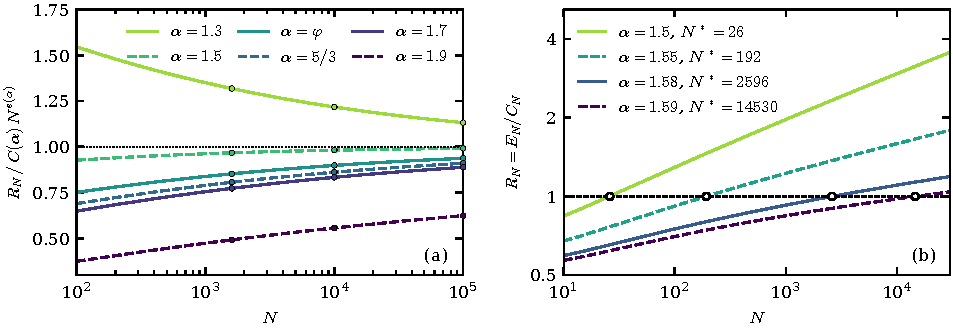
\includegraphics{figures/heavy}
\caption{Alternating runs with $\Prob(L\ge k)=k^{-\alpha}$ and a
stationary start. (a) The ratio $R_n=E_n/C_n$ divided by its asymptotic
form $C(\alpha)n^{e(\alpha)}$ from Corollary~\ref{cor:golden}, for even $n$
from 100 to $10^5$. The dots are the entries of Table~\ref{tab:heavy}.
(b) $R_n$ for 4 values of $\alpha$ just below the golden ratio. On the
computed range $10\le n\le3\cdot10^4$ each curve crosses 1 once, at
$n^*(\alpha)$ (circles).}
\label{fig:heavy}
\end{figure}

For $\alpha\ge2$ the sums $\tau_m$ have a Gaussian limit, and the center
wins with either start.

\begin{theorem}[$\alpha\ge2$]\label{thm:alpha2}
Let $D$ be any a.s.\ finite first run.
\begin{enumerate}[(a)]
\item If $\alpha>2$, let
$v=\Var L=2\zeta(\alpha-1)-\zeta(\alpha)-\zeta(\alpha)^2$. Then
$C_n\sim\sqrt{2\mu/(\pi vn)}$, and with a stationary start
$R_n\sim C_2(\alpha)n^{3/2-\alpha}$, where
$C_2(\alpha)=\sqrt{\pi v/(2\mu)}\big/(2(\alpha-1)\mu)$.
\item If $\alpha=2$, then $C_n\sim\sqrt{2\mu/(\pi n\log n)}$, and with a
stationary start $R_n\sim\sqrt{\pi\log n/(8\zeta(2)^3n)}$.
\end{enumerate}
\end{theorem}

The proof is in Appendix~\ref{app:heavy}. The exponent of $R_n$ is
continuous at $\alpha=2$, since $e(2)=-\frac12=\frac32-2$. At $\alpha=2$,
$R_n$ divided by the leading term of (b) is $0.885$ at $n=1600$ and $0.943$ at
$n=10^5$, which is consistent with a correction of order $1/\log n$.

For $0<\alpha<1$ the runs have infinite mean and only the fresh start makes
sense. Then the center is of order $1/n$.

\begin{theorem}[$0<\alpha<1$]\label{thm:lamperti}
Let $0<\alpha<1$, with a fresh start. Then
$nC_n\to\ell_\alpha(\frac12)=\frac2\pi\tan\frac{\pi\alpha}2$, where
\[
 \ell_\alpha(y)=\frac{\sin\pi\alpha}{\pi}\,
 \frac{y^{\alpha-1}(1-y)^{\alpha-1}}{y^{2\alpha}+2y^\alpha(1-y)^\alpha
 \cos\pi\alpha+(1-y)^{2\alpha}}\qquad(0<y<1)
\]
is the density of Lamperti's occupation-time law
\cite{lamperti1958,godrecheluck2001}. Hence
$R_n\sim\frac{\pi}{4\tan(\pi\alpha/2)}n^{1-\alpha}\to\infty$, and the ends
win for every $\alpha<1$. The point $y=\frac12$ is a strict local minimum of
$\ell_\alpha$ for $\alpha<\alpha_c$ and a strict local maximum for
$\alpha>\alpha_c$, where $\alpha_c=0.5946116441$ is the root of
$\alpha=\cos(\pi\alpha/2)$.
\end{theorem}

The proof is in Appendix~\ref{app:heavy}. The critical value $\alpha_c$ is in
\cite[Section~7]{godrecheluck2001}, below eq.~(7.6). We do not prove the
global shape of $\ell_\alpha$ (the U and W shapes
in~\cite{godrecheluck2001,zdk2015}),
and we do not prove that the center bin at finite $n$ is a local minimum or
maximum of the law of $A_n$. At $n=16000$ it is a local minimum for
$\alpha=0.58$ and a local maximum for $\alpha=0.61$, but the relative second
differences are only about $4\cdot10^{-9}$ and $2\cdot10^{-9}$.

\begin{remark}[the fresh start]\label{rem:fresh}
With a fresh start the threshold is $\alpha=1$. The ends win for $\alpha<1$
by Theorem~\ref{thm:lamperti}, and the center wins for $\alpha>1$ by
Corollary~\ref{cor:golden} and Theorem~\ref{thm:alpha2}. At $\alpha=1$ we
only have a heuristic. Suppose we repeat the proof of
Theorem~\ref{thm:center} with a skewed Cauchy limit, the centering
$m(H_{m+1}-1)$ and the density $1/\pi^2$ at $0$ of the difference of 2
copies of the limit. This suggests
$R_n\approx\pi^2\tilde m_h/(8h)\sim\pi^2/(8\log n)$, where $\tilde m_h$
solves $m(H_{m+1}-1)=h$. We have not controlled the error terms, so the claim that
the center wins by a logarithm is not proved. The exact $R_n$ divided by
$\pi^2\tilde m_h/(8h)$ is $0.796$, $0.850$ and $0.886$ at $n=1600$, $10^4$ and
$10^5$. Below $\alpha=1$ the crossover can be late. Setting the limit form in
Theorem~\ref{thm:lamperti} equal to $1$ gives
$n\approx(4\tan(\pi\alpha/2)/\pi)^{1/(1-\alpha)}$, which is $21$ at
$\alpha=0.7$ and $1.1\cdot10^9$ at $\alpha=0.9$. Indeed $R_{16000}=0.59$ at
$\alpha=0.9$.
\end{remark}

\begin{remark}[crossover sizes]\label{rem:crossover}
For $\alpha<\varphi$ and a stationary start, $R_n\to\infty$ by
Corollary~\ref{cor:golden}. But when
$\alpha$ is close to $\varphi$, $R_n<1$ for small $n$ and the crossover is
late. For $\alpha=1.5,1.55,1.58,1.59$ we computed $R_n$ for every even $n$
with $10\le n\le3\cdot10^4$. In each case $R_n-1$ changes sign once, at
$n^*(\alpha)=26,192,2596,14530$, where $n^*(\alpha)$ is the even $n$ with
$R_{n-2}<1<R_n$. At $\alpha=1.60$ a 30-point grid on
$[3\cdot10^4,4.2\cdot10^5]$ and then bisection over even $n$ give
$n^*(1.60)=372660$. These are the last sign changes in the computed range,
and we have no bound that rules out a later one. The leading order
$C(\alpha)^{-1/e(\alpha)}$ underestimates them by factors $1.9$ to $7.4$.
Heuristically, setting $C(\alpha)n^{e(\alpha)}=1$ and using
$e(\alpha)\approx(\sqrt5/\varphi)(\varphi-\alpha)$ gives
$\log n^*(\alpha)=0.1834/(\varphi-\alpha)+O(1)$ as $\alpha\uparrow\varphi$,
where $0.1834=\varphi\lvert\log C(\varphi)\rvert/\sqrt5$. At the 5 values of
$\alpha$ above, the $O(1)$ term is $1.7$ to $3.0$. A proof would need
Theorem~\ref{thm:center}, with its correction terms, to hold uniformly in
$\alpha$ near $\varphi$.
\end{remark}

\begin{remark}[heat conduction]\label{rem:heat}
L\'evy-walk models of anomalous heat conduction use $\alpha=5/3$
\cite{dsd2013,zdk2015}. Then $e(5/3)=-\frac1{15}$, and with a stationary
start $R_n\sim0.8351\,n^{-1/15}$. The approach is slow and not monotone. On
even $n$ in $[20,400]$, $R_n$ increases up to $n=150$, where
$R_{150}=0.42419$, and after that it decreases on the computed grid, with
$R_n/(C(5/3)n^{-1/15})=0.910$ at $n=10^5$. In the L\'evy-walk model the
flights choose their directions independently. So a maximal run is a sum of
a geometric number of flights and has the same tail exponent, and the exponent
$-\frac1{15}$ should carry over with a different constant. We have not proved
this. In that model the 2 starts also have to be kept apart. Dhar, Saito and
Derrida~\cite{dsd2013} write the equation for a fresh start, where the end
atom is of order $t^{-\alpha}$, but quote the peak size $t^{1-\alpha}$ of the
equilibrium start (their $\beta$ is our $\alpha$).
\end{remark}

The last walk has aging memory. As for $\alpha<1$, its fraction of $+$ steps
has a limit law, so its center is of order $1/n$.

\begin{remark}[aging]\label{rem:aging}
Let the walk take a fair first step and then switch direction at step $k\ge2$
with probability $c/k$, where $0<c<2$. Dietz and Sethuraman proved that
$A_n/n$ converges in law to $\mathrm{Beta}(c,c)$
\cite[Example~1.1 and Theorem~1.4]{ds2007}. For $c\le1$ their chain is
exactly this walk. Engl\"ander and Volkov gave a different proof
\cite[Theorem~1]{ev2018}. The limit is uniform exactly when $c=1$
\cite[Remark~2]{ev2018}. Fix the first step at $+1$. At $c=1$, $A_n$ is then
exactly uniform on $\{1,\dots,n\}$ for every $n$
(Appendix~\ref{app:aging}). A path with $A_n=s<n$
switches at least once, and a switch at time $t$ multiplies the path
probability by the odds $\omega_t=c/(t-c)$, which increase in $c$. So
$\Prob_+(A_n=s)/\Prob_+(A_n=n)$ increases strictly in $c$ for $1\le s\le n-1$
and equals $1$ at $c=1$, and the fixed-start crossing is exactly $c=1$ for
every $n$ and every bin. With a fair first step each end is $\frac1{2n}$ at
$c=1$ while every interior bin is $\frac1n$. By the same argument $C_n/E_n$
increases strictly in $c$ and tends to $0$ as $c\to0$. So the crossing $c_n$
is unique and below $1$. For
even $n$,
\[
 c_n=1-\frac{\log2}{\log n+\gamma+2-2\log2}+O\bigl((\log n)^{-3}\bigr).
\]
For example, computed to high precision, $c_{200}=0.8925$ and
$c_{800}=0.9116$. The $\log2$ comes from the fair start under switching
probability $c/k$, and not from aging. With switching probability $c/(k+1)$
and a fair start, $A_n$ is exactly uniform on $\{0,\dots,n\}$ at $c=1$
(Appendix~\ref{app:aging}). A switch at time $t$ then has the odds
$c/(t+1-c)$, which also increase in $c$, so this crossing is exactly $c=1$
for every $n$. The proof, in Appendix~\ref{app:aging}, compares
the end, which is exactly $\frac12\prod_{k=2}^n(1-c/k)$ and of order $n^{-c}$,
with a local limit theorem at the center.
\end{remark}
